\documentclass[journal,12pt,twocolumn]{IEEEtran}
\usepackage{setspace}
\usepackage{gensymb}
\usepackage{caption}
%\usepackage{multirow}
%\usepackage{multicolumn}
%\usepackage{subcaption}
%\doublespacing
\singlespacing
\usepackage{csvsimple}
\usepackage{amsmath}
\usepackage{multicol}
%\usepackage{enumerate}
\usepackage{amssymb}
%\usepackage{graphicx}
\usepackage{newfloat}
%\usepackage{syntax}
\usepackage{listings}
\usepackage{tikz}
\usetikzlibrary{shapes,arrows}



%\usepackage{graphicx}
%\usepackage{amssymb}
%\usepackage{relsize}
%\usepackage[cmex10]{amsmath}
%\usepackage{mathtools}
%\usepackage{amsthm}
%\interdisplaylinepenalty=2500
%\savesymbol{iint}
%\usepackage{txfonts}
%\restoresymbol{TXF}{iint}
%\usepackage{wasysym}
\usepackage{amsthm}
\usepackage{mathrsfs}
\usepackage{txfonts}
\usepackage{stfloats}
\usepackage{cite}
\usepackage{cases}
\usepackage{mathtools}
\usepackage{caption}
\usepackage{enumerate}	
\usepackage{enumitem}
\usepackage{amsmath}
%\usepackage{xtab}
\usepackage{longtable}
\usepackage{multirow}
%\usepackage{algorithm}
%\usepackage{algpseudocode}
\usepackage{enumitem}
\usepackage{mathtools}
\usepackage{hyperref}
%\usepackage[framemethod=tikz]{mdframed}
\usepackage{listings}
    %\usepackage[latin1]{inputenc}                                 %%
    \usepackage{color}                                            %%
    \usepackage{array}                                            %%
    \usepackage{longtable}                                        %%
    \usepackage{calc}                                             %%
    \usepackage{multirow}                                         %%
    \usepackage{hhline}                                           %%
    \usepackage{ifthen}                                           %%
  %optionally (for landscape tables embedded in another document): %%
    \usepackage{lscape}     


\usepackage{url}
\def\UrlBreaks{\do\/\do-}


%\usepackage{stmaryrd}


%\usepackage{wasysym}
%\newcounter{MYtempeqncnt}
\DeclareMathOperator*{\Res}{Res}
%\renewcommand{\baselinestretch}{2}
\renewcommand\thesection{\arabic{section}}
\renewcommand\thesubsection{\thesection.\arabic{subsection}}
\renewcommand\thesubsubsection{\thesubsection.\arabic{subsubsection}}

\renewcommand\thesectiondis{\arabic{section}}
\renewcommand\thesubsectiondis{\thesectiondis.\arabic{subsection}}
\renewcommand\thesubsubsectiondis{\thesubsectiondis.\arabic{subsubsection}}

% correct bad hyphenation here
\hyphenation{op-tical net-works semi-conduc-tor}

%\lstset{
%language=C,
%frame=single, 
%breaklines=true
%}

%\lstset{
	%%basicstyle=\small\ttfamily\bfseries,
	%%numberstyle=\small\ttfamily,
	%language=Octave,
	%backgroundcolor=\color{white},
	%%frame=single,
	%%keywordstyle=\bfseries,
	%%breaklines=true,
	%%showstringspaces=false,
	%%xleftmargin=-10mm,
	%%aboveskip=-1mm,
	%%belowskip=0mm
%}

%\surroundwithmdframed[width=\columnwidth]{lstlisting}
\def\inputGnumericTable{}                                 %%
\lstset{
%language=C,
frame=single, 
breaklines=true,
columns=fullflexible
}
 

\begin{document}
%
\tikzstyle{block} = [rectangle, draw,
    text width=3em, text centered, minimum height=3em]
\tikzstyle{sum} = [draw, circle, node distance=3cm]
\tikzstyle{input} = [coordinate]
\tikzstyle{output} = [coordinate]
\tikzstyle{pinstyle} = [pin edge={to-,thin,black}]

\theoremstyle{definition}
\newtheorem{theorem}{Theorem}[section]
\newtheorem{problem}{Problem}
\newtheorem{proposition}{Proposition}[section]
\newtheorem{lemma}{Lemma}[section]
\newtheorem{corollary}[theorem]{Corollary}
\newtheorem{example}{Example}[section]
\newtheorem{definition}{Definition}[section]
%\newtheorem{algorithm}{Algorithm}[section]
%\newtheorem{cor}{Corollary}
\newcommand{\BEQA}{\begin{eqnarray}}
\newcommand{\EEQA}{\end{eqnarray}}
\newcommand{\define}{\stackrel{\triangle}{=}}
\bibliographystyle{IEEEtran}
%\bibliographystyle{ieeetr}
\providecommand{\nCr}[2]{\,^{#1}C_{#2}} % nCr
\providecommand{\nPr}[2]{\,^{#1}P_{#2}} % nPr
\providecommand{\mbf}{\mathbf}
\providecommand{\pr}[1]{\ensuremath{\Pr\left(#1\right)}}
\providecommand{\qfunc}[1]{\ensuremath{Q\left(#1\right)}}
\providecommand{\sbrak}[1]{\ensuremath{{}\left[#1\right]}}
\providecommand{\lsbrak}[1]{\ensuremath{{}\left[#1\right.}}
\providecommand{\rsbrak}[1]{\ensuremath{{}\left.#1\right]}}
\providecommand{\brak}[1]{\ensuremath{\left(#1\right)}}
\providecommand{\lbrak}[1]{\ensuremath{\left(#1\right.}}
\providecommand{\rbrak}[1]{\ensuremath{\left.#1\right)}}
\providecommand{\cbrak}[1]{\ensuremath{\left\{#1\right\}}}
\providecommand{\lcbrak}[1]{\ensuremath{\left\{#1\right.}}
\providecommand{\rcbrak}[1]{\ensuremath{\left.#1\right\}}}
\theoremstyle{remark}
\newtheorem{rem}{Remark}
\newcommand{\sgn}{\mathop{\mathrm{sgn}}}
\providecommand{\abs}[1]{\left\vert#1\right\vert}
\providecommand{\res}[1]{\Res\displaylimits_{#1}} 
\providecommand{\norm}[1]{\left\Vert#1\right\Vert}
\providecommand{\mtx}[1]{\mathbf{#1}}
\providecommand{\mean}[1]{E\left[ #1 \right]}
\providecommand{\fourier}{\overset{\mathcal{F}}{ \rightleftharpoons}}
%\providecommand{\hilbert}{\overset{\mathcal{H}}{ \rightleftharpoons}}
\providecommand{\system}{\overset{\mathcal{H}}{ \longleftrightarrow}}
	%\newcommand{\solution}[2]{\textbf{Solution:}{#1}}
\newcommand{\solution}{\noindent \textbf{Solution: }}
\newcommand{\myvec}[1]{\ensuremath{\begin{pmatrix}#1\end{pmatrix}}}
\providecommand{\dec}[2]{\ensuremath{\overset{#1}{\underset{#2}{\gtrless}}}}
\DeclarePairedDelimiter{\ceil}{\lceil}{\rceil}
%\numberwithin{equation}{section}
%\numberwithin{problem}{subsection}
%\numberwithin{definition}{subsection}
\makeatletter
\@addtoreset{figure}{section}
\makeatother
\let\StandardTheFigure\thefigure
%\renewcommand{\thefigure}{\theproblem.\arabic{figure}}
\renewcommand{\thefigure}{\thesection}
%\numberwithin{figure}{subsection}
%\numberwithin{equation}{subsection}
%\numberwithin{equation}{section}
%\numberwithin{equation}{problem}
%\numberwithin{problem}{subsection}
\numberwithin{problem}{section}
%%\numberwithin{definition}{subsection}
%\makeatletter
%\@addtoreset{figure}{problem}
%\makeatother
\makeatletter
\@addtoreset{table}{section}
\makeatother
\let\StandardTheFigure\thefigure
\let\StandardTheTable\thetable
\let\vec\mathbf
\numberwithin{equation}{section}
\vspace{3cm}
\title{%Convex Optimization in Python
	\logo{
	Random Numbers
	}
}
%\title{
%	\logo{Matrix Analysis through Octave}{\begin{center}\includegraphics[scale=.24]{tlc}\end{center}}{}{HAMDSP}
%}
% paper title
% can use linebreaks \\ within to get better formatting as desired
%\title{Matrix Analysis through Octave}
%
%
% author names and IEEE memberships
% note positions of commas and nonbreaking spaces ( ~ ) LaTeX will not break
% a structure at a ~ so this keeps an author's name from being broken across
% two lines.
% use \thanks{} to gain access to the first footnote area
% a separate \thanks must be used for each paragraph as LaTeX2e's \thanks
% was not built to handle multiple paragraphs
%
\author{AI21BTECH11016}
\maketitle
\tableofcontents
\bigskip
\renewcommand{\thefigure}{\theenumi}
\renewcommand{\thetable}{\theenumi}
\section{Uniform Random Numbers}
Let $U$ be a uniform random variable between 0 and 1.
\begin{enumerate}[label=\thesection.\arabic*
,ref=\thesection.\theenumi]
\item Generate $10^6$ samples of $U$ using a C program and save into a file called uni.dat .
\\
\solution
\begin{lstlisting}
https://github.com/JBA-12/Sim-Assignment1/blob/main/codes/1.1.c
https://github.com/JBA-12/Sim-Assignment1/blob/main/codes/coeffs.h
\end{lstlisting}
Run the code using the following commands
\begin{lstlisting}
gcc -o out 1.1.c coeffs.h -lm
./out
\end{lstlisting}
This generates an output file "uni.dat".\\
%
\item
Load the uni.dat file into python and plot the empirical CDF of $U$ using the samples in uni.dat. The CDF is defined as
\begin{align}
F_{U}(x) = \pr{U \le x}
\end{align}
\\
\solution  The following code plots Fig. \ref{fig:uni_cdf}
\begin{lstlisting}
https://github.com/JBA-12/Sim-Assignment1/blob/main/codes/1.2.py
\end{lstlisting}
and run the code using the following command
\begin{lstlisting}
python3 1.2.py
\end{lstlisting}
\begin{figure}[!htbp]
\centering
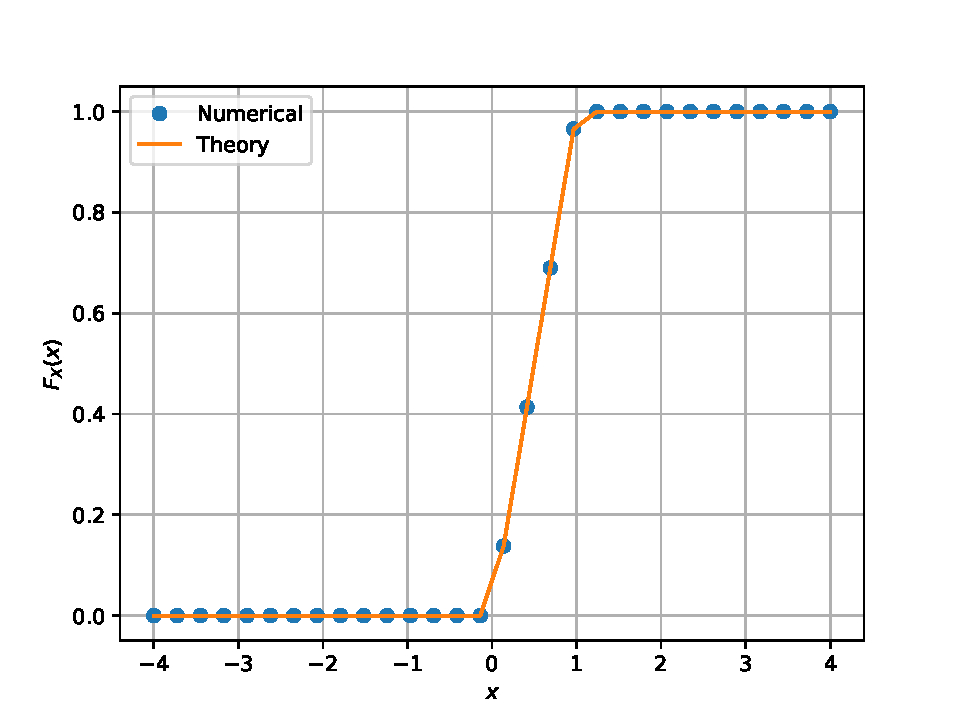
\includegraphics[width=\columnwidth]{./figs/uni_cdf}
\caption{The CDF of $U$}
\label{fig:uni_cdf}
\end{figure}
%
\item
Find a  theoretical expression for $F_{U}(x)$.\\
\solution 
$F_{U}(x)$ is given by
\begin{align}
F_{U}(x) = \pr{U \le x} = \int_{-\infty}^{x} p_{U}(u)du \\
PDF function : p_{U}(u) =
    \begin{cases}
       1, & u \in (0,1) \\
       0, & otherwise
    \end{cases}  
\end{align}
\begin{align}
if x<0 : \int_{-\infty}^{x} p_U(x) dx & = 0\\ \because p_U(x) & = 0
\end{align}
\begin{align}
if 0\leq x \leq1 :\\ \int_{-\infty}^{x} p_U(x) dx & = \int_{-\infty}^{0} p_U(x) dx + \int_{0}^{x} p_U(x) dx\\& = \int_{-\infty}^{0} 0 dx + \int_{0}^{x} 1 dx\\& = 0+x\\& = x
\end{align}
\begin{align}
if x>1 :\\ \int_{-\infty}^{x} p_U(x) dx \\& = \int_{-\infty}^{0} p_U(x) dx + \int_{0}^{x} p_U(x) dx + \int_{1}^x p_U(x) dx\\ & = \int_{-\infty}^{0} 0 dx + \int_{0}^{1} 1 dx + \int_{1}^x 0 dx\\& = 0+1+0\\& = 1
\end{align}
\begin{align}
\Rightarrow F_{U}(x) & =   
   \begin{cases}
       0, & x \in (-\infty,0) \\
       x, & x \in (0,1) \\
       1, & x \in (1,\infty)
    \end{cases} 
\end{align}
\item
The mean of $U$ is defined as
%
\begin{equation}
E\sbrak{U} = \frac{1}{N}\sum_{i=1}^{N}U_i
\end{equation}
%
and its variance as
%
\begin{equation}
\text{var}\sbrak{U} = E\sbrak{U- E\sbrak{U}}^2 
\end{equation}
Write a C program to  find the mean and variance of $U$. \\
\solution 
\begin{lstlisting}
https://github.com/JBA-12/Sim-Assignment1/blob/main/codes/1.4.c
https://github.com/JBA-12/Sim-Assignment1/blob/main/codes/coeffs.h
\end{lstlisting}
Run the code using the following commands 
\begin{lstlisting}
gcc -o out 1.4.c coeffs.h -lm
./out
\end{lstlisting}
\item Verify your result theoretically given that
\end{enumerate}
%
\begin{equation}
E\sbrak{U^k} = \int_{-\infty}^{\infty}x^kdF_{U}(x)
\end{equation}
\solution
From 1.4 we have,
\begin{align}
dF_{U}(x) & =   
   \begin{cases}
       0, & x \in (-\infty,0) \\
       dx, & x \in (0,1) \\
       0, & x \in (1,\infty)
    \end{cases}\\
E\sbrak{U} & = \int_{-\infty}^{\infty}x dF_{U}(x) \\
E\sbrak{U} & = \int_{0}^{1} xdx = \frac{1}{2}
\end{align}
\begin{align}
E\sbrak{U^2} = \int_{-\infty}^{\infty}x^2 dF_{U}(x) \\
E\sbrak{U} = \int_{0}^{1} x^2 dx = \frac{1}{3}\\
variance = E\sbrak{U^2} - {E\sbrak{U}}^2\\ = \frac{1}{3} - \frac{1}{4} = \frac{1}{12}
\end{align}
\section{Central Limit Theorem}
%
\begin{enumerate}[label=\thesection.\arabic*
,ref=\thesection.\theenumi]
%
\item
Generate $10^6$ samples of the random variable
%
\begin{equation}
X = \sum_{i=1}^{12}U_i -6
\end{equation}
%
using a C program, where $U_i, i = 1,2,\dots, 12$ are  a set of independent uniform random variables between 0 and 1
and save in a file called gau.dat\\
\solution
\begin{lstlisting}
https://github.com/JBA-12/Sim-Assignment1/blob/main/codes/2.1.c
https://github.com/JBA-12/Sim-Assignment1/blob/main/codes/coeffs.h
\end{lstlisting}
Run the code using the following commands
\begin{lstlisting}
gcc -o out 2.1.c coeffs.h -lm
./out
\end{lstlisting}
This generates an output file "gau.dat".\\
\item
Load gau.dat in python and plot the empirical CDF of $X$ using the samples in gau.dat. What properties does a CDF have?
\\
\solution The CDF of $X$ is plotted in Fig. \ref{fig:gauss_cdf} \\\\
Uncomment the Question-2.2 of following python file
\begin{lstlisting}
https://github.com/JBA-12/Sim-Assignment1/blob/main/codes/2.2.py
\end{lstlisting}
and run the code using the following command
\begin{lstlisting}
python3 2.2.py
\end{lstlisting}
\begin{figure}[!htbp]
\centering
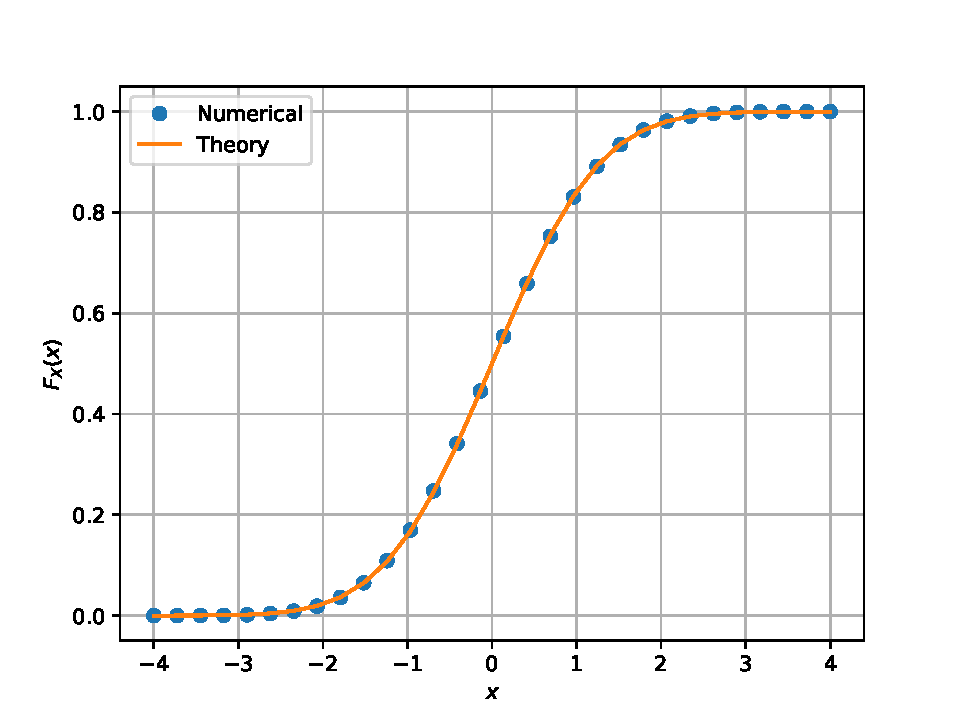
\includegraphics[width=\columnwidth]{./figs/gau_cdf}
\caption{The CDF of $X$}
\label{fig:gauss_cdf}
\end{figure}
\item
Load gau.dat in python and plot the empirical PDF of $X$ using the samples in gau.dat. The PDF of $X$ is defined as
\begin{align}
p_{X}(x) = \frac{d}{dx}F_{X}(x)
\end{align}
What properties does the PDF have?
\\
\solution The PDF of $X$ is plotted in Fig. \ref{fig:gauss_pdf} using the code below
\begin{lstlisting}
wget https://github.com/gadepall/probability/raw/master/manual/codes/2.3.py
\end{lstlisting}
and run the code using the following command
\begin{lstlisting}
python3 2.3.py
\end{lstlisting}
\begin{figure}[!htbp]
\centering
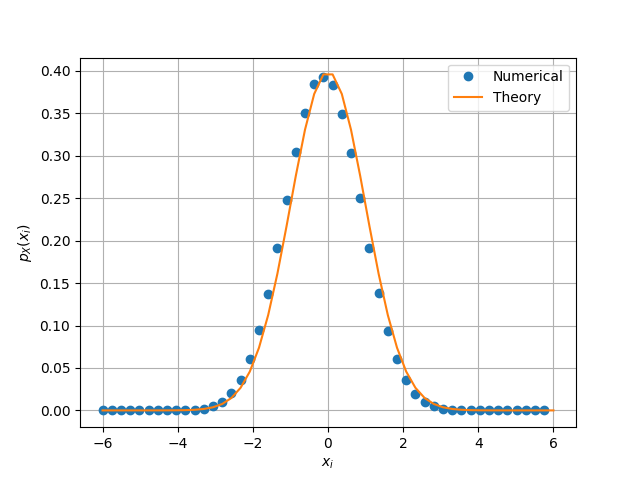
\includegraphics[width=\columnwidth]{./figs/gauss_pdf}
\caption{The PDF of $X$}
\label{fig:gauss_pdf}
\end{figure}
\item Find the mean and variance of $X$ by writing a C program.\\
\solution 
\begin{lstlisting}
https://github.com/JBA-12/Sim-Assignment1/blob/main/codes/2.4.c
https://github.com/JBA-12/Sim-Assignment1/blob/main/codes/coeffs.h
\end{lstlisting}
and run the following commands 
\begin{lstlisting}
gcc -o out 2.4.c coeffs.h -lm
./out
\end{lstlisting}
\item Given that 
\begin{align}
p_{X}(x) = \frac{1}{\sqrt{2\pi}}\exp\brak{-\frac{x^2}{2}}, -\infty < x < \infty,
\end{align}
repeat the above exercise theoretically.\\
\solution 
\begin{align}
E\sbrak{X} & = \int_{-\infty}^{\infty}x dF_{U}(x)\\
E\sbrak{X} & = \int_{-\infty}^{\infty}x \frac{1}{\sqrt{2\pi}}\exp\brak{-\frac{x^2}{2}}dx\\ & = \sbrak{-\frac{1}{\sqrt{2\pi}}\exp\brak{-\frac{x^2}{2}}}_{-\infty}^{\infty}\\ & = 0
\end{align}
\begin{align}
E\sbrak{X^2} & = \int_{-\infty}^{\infty}x^2 dF_{U}(x) \\
E\sbrak{X^2} & = \int_{-\infty}^{\infty}x^2 \frac{1}{\sqrt{2\pi}}\exp\brak{-\frac{x^2}{2}}dx\\& = \frac{1}{\sqrt{2\pi}} \int_{-\infty}^{\infty} 2x^2 \exp\brak{-x^2} \sqrt{2}dx\\& = 1
\end{align}
\begin{align}
\because \int_{-\infty}^{\infty} x^2 \exp{-x^2}dx = \frac{\sqrt{\pi}}{2}\\
variance = E\sbrak{X^2} - {E\sbrak{X}}^2\\ = 1-0 \\ = 1
\end{align}
%
\end{enumerate}
\section{From Uniform to Other}
\begin{enumerate}[label=\thesection.\arabic*
,ref=\thesection.\theenumi]
%
\item
Generate samples of 
%
\begin{equation}
V = -2\ln\brak{1-U}
\end{equation}
%
and plot its CDF. \\
\solution
\begin{lstlisting}
https://github.com/JBA-12/Sim-Assignment1/blob/main/codes/3.1.c
https://github.com/JBA-12/Sim-Assignment1/blob/main/codes/coeffs.h
\end{lstlisting}
and run the code using the following commands
\begin{lstlisting}
gcc -o out 3.1.c coeffs.h -lm
./out
\end{lstlisting}
This generates an output file "V.dat".\\\\
Plotting cdf for V:\\
The following code plots Fig. \ref{fig:uni_cdf}\\\\

\begin{lstlisting}
https://github.com/JBA-12/Sim-Assignment1/blob/main/codes/3.1.py
\end{lstlisting}
and run the code using the following command
\begin{lstlisting}
python3 3.1.py
\end{lstlisting}
\begin{figure}[!htbp]
\centering
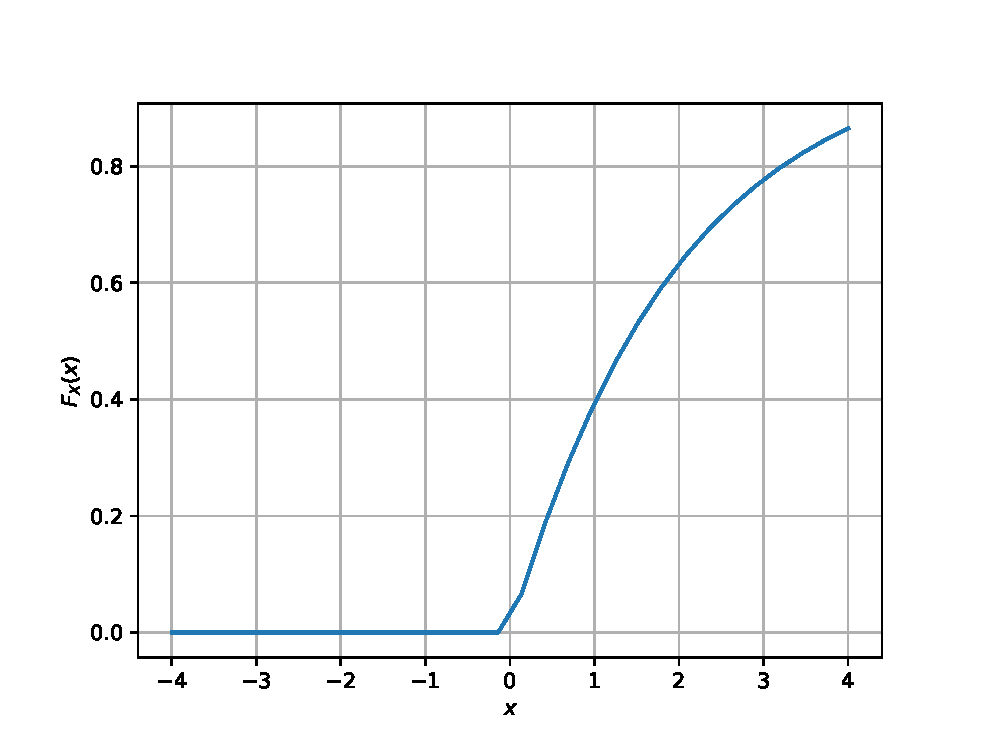
\includegraphics[width=\columnwidth]{./figs/v_cdf}
\caption{The CDF of $U$}
\label{fig:V_cdf}
\end{figure}
\item Find a theoretical expression for $F_V(x)$.\\
\solution
\begin{align}
F_V(x) & = \pr{V \leq x}\\& = \pr{-2ln(1-U) \leq x}\\& = \pr{ln(1-U) \geq \frac{-x}{2}}\\& = \pr{1-U \geq \exp\brak{-\frac{x}{2}}}\\& = \pr{U \leq 1-\exp\brak{-\frac{x}{2}}}\\& = F_U{\brak{1-\exp\brak{-\frac{x}{2}}}}
\end{align}
Here we have :\\
\begin{align}
0 \le 1-\exp\brak{-\frac{x}{2}} &< 1 \qquad \text{if } x \ge 0	\\	
		1-\exp\brak{-\frac{x}{2}} &< 0 \qquad \text{if } x < 0	
\end{align}
\begin{align}
\therefore F_V(x) = 
		\begin{cases}
			0 & x < 0\\
			1-\exp\brak{-\frac{x}{2}} & x \geq 0 
		\end{cases}
\end{align}
%
%\item
%Generate the Rayleigh distribution from Uniform. Verify your result through graphical plots.
\end{enumerate}
\end{document}